\section{Hello World}

\paragraph{}
   In this part of the document, we're going to be touching on one of the foundational elements in teaching the C programming language: the `Hello World'
   program. Simply put, we are going to write a program that prints the line ``Hello, world!'' into the terminal where we can see it. For the sake of
   simplicity, each figure in this document will be done in Visual Studio Code, but I will, from time to time, include examples from other editors to
   show what may need to be done differently to achieve the same or similar result.

\paragraph{}
   In order to accomplish this, we must first open our text editor and our command line interface (terminal) if they aren't already open. With those
   programs up and running, we must create the file that our code will reside in:

\begin{figure}[h!]
   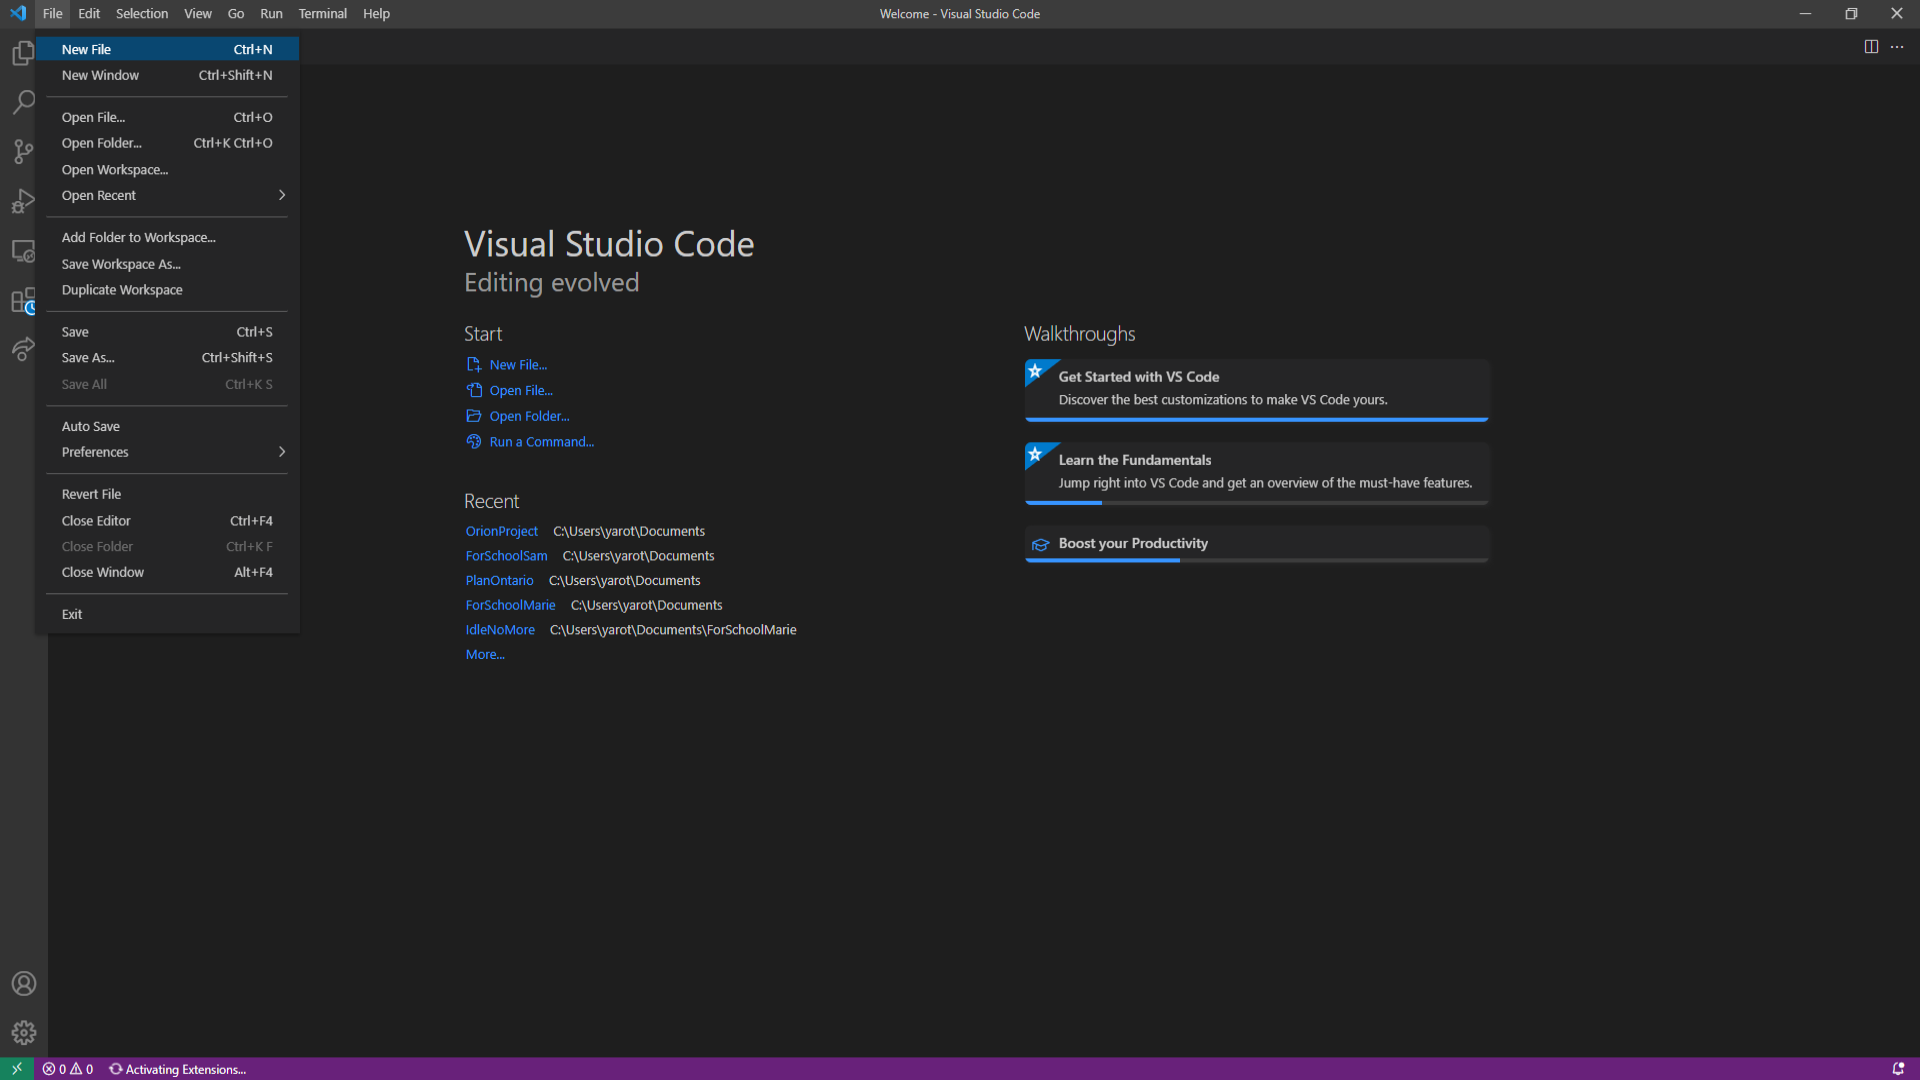
\includegraphics[width=\linewidth]{Figure1_VSCODE.png}
   \caption{Create the file by clicking on the ``New File'' button.}
   \label{fig:vscode_newfile}
\end{figure}

\paragraph{}
   Once the new file is created, we can begin by writing a few lines of code. Don't worry if the figure below is confusing as we will explain each
   individual line as we continue.

% A \newpage is necessary here to avoid splitting the figure in half.
\newpage

\begin{lstlisting}
// https://github.com/mnimi/intro_to_programming/tree/trunk/examples/clang/hello_world/main.c

#include <stdio.h>

int main()
{
   printf("Hello, world!");

   return 0;
}
\end{lstlisting}

\paragraph{}
   Alright, let's begin with line one. The two forward-slashes represent a single-line comment. These are used to relay information to any individual
   reading the source code of a program. These should be used as often as possible in your code in order to convey the purpose of every action your
   program performs. In this case, the comment conveys where you can find this file.

\paragraph{}
   Line two is just blank space. Most of your files will consist of blank space on some level depending on how you format your code.

\paragraph{}
   Line three is where things get somewhat interesting. This is an include statement. The `\#' symbol denotes a preprocessor directive, which tells
   the C compiler to perform an action, which in this case is to include a file from the standard C library called ``stdio.h''. This is a header file
   that contains some very important functionality relating to system input and output, something that we will go into more detail on in a later
   section.

\paragraph{}
   On line five, we begin to see some operational details of our program in the form of the \textit{main} function's return type and name. Here, we
   are returning an \textit{int}, which represents an integer in C.

\paragraph{}
   When we get to line six, you might notice something slightly strange. A curly brace and then a newline. Why is this here? Well, in C and languages
   that descend from C, curly braces often denote the \textit{scope} of an operation or set of operations. This is useful because it tells the
   programmer and the compiler where a function or other instructions start and where they end. Something important to remember is that every function
   that you write will require at least one set of these or more depending on the kind of instructions that your function contain.

\paragraph{}
   One line lower, we see our first \textit{function call}. This is us utilizing a function that comes from the \textit{stdio.h} header called `printf'.
   `printf' can take a number of arguments, but only one that we will discuss right now: a `constant pointer to a char', or \textit{const char*}.

\paragraph{}
   Finally, we reach line nine, where we see a `return' statement. This tells the compiler that when we reach this point in the program, it is to exit
   with a \textit{return code} of zero, which denotes that no errors occurred during the run-time of our program.

\paragraph{}
   With these things in mind, we are going to continue into our next chapter: \textit{data types}. Some things important to remember include the idea
   of commenting as much as you can as well as using curly braces to denote the scope of actions you take in your program.

% A \newpage should be placed at the end of every section.
\newpage
